\documentclass[12pt]{article}

\usepackage{fullpage}
\usepackage{graphicx, rotating, booktabs} 
\usepackage{times} 
\usepackage{natbib} 
\usepackage{indentfirst} 
\usepackage{setspace}
\usepackage{grffile} 
\usepackage{hyperref}
\usepackage{adjustbox}
\setcitestyle{aysep{}}


\singlespace
\title{\textbf{Appendix to Paper: Arms, Alliances and Alliance Treaty Design}}
\author{Joshua Alley\footnote{Graduate Student,
Department of Political Science, Texas A\&M University.}}
\date{{\normalsize \today}}

\bibliographystyle{apsr}

\begin{document}

\maketitle 

\doublespace 



\section{Priors}

\autoref{tab:priors} summarizes the prior distributions in the multilevel model. 
All these priors are meant to be weakly informative relative to the scale of the data. 
$\nu$ is the degrees of freedom for the t-distribution, and the gamma prior is the recommended default prior for STAN. 

\begin{table} % Create a table of priors.
\begin{center}
\begin{tabular}{c} 
$ p(\alpha) \sim N(0, 1)$  \\
$ p(\sigma) \sim \mbox{half-}N(0, 1) $ \\
$ p(\alpha^{yr}) \sim N(0, \sigma^{yr}) $ \\ 
$ p(\sigma^{yr}) \sim N(0, 1) $ \\
$ p(\alpha^{st}) \sim N(0, \sigma^{st}) $ \\ 
$ p(\sigma^{st}) \sim \mbox{half-}N(0, 1) $ \\ 
$ p(\sigma^{all}) \sim \mbox{half-}N(0, 1) $ \\
$ p(\beta) \sim N(0, 1) $ \\
$ p(\gamma) \sim N(0, 1) $ \\ 
$ p(\nu) \sim gamma(2, 0.1)$ 
\end{tabular} 
\caption{Summary of Priors in Multilevel Model} 
\label{tab:priors}
\end{center} 
\end{table} 


\section{HMC Diagnostics}

There were no divergent iterations running 4 chains for 2,000 iterations in either sample. The $\hat{R}$ is less than 1.1 for all parameters in both samples. 

Trace plots in \autoref{fig:trace-all-min} and \autoref{fig:trace-all-maj} indicate good mixing of the chains for the alliance-level parameters. 

\begin{figure}[htbp]
	\centering
		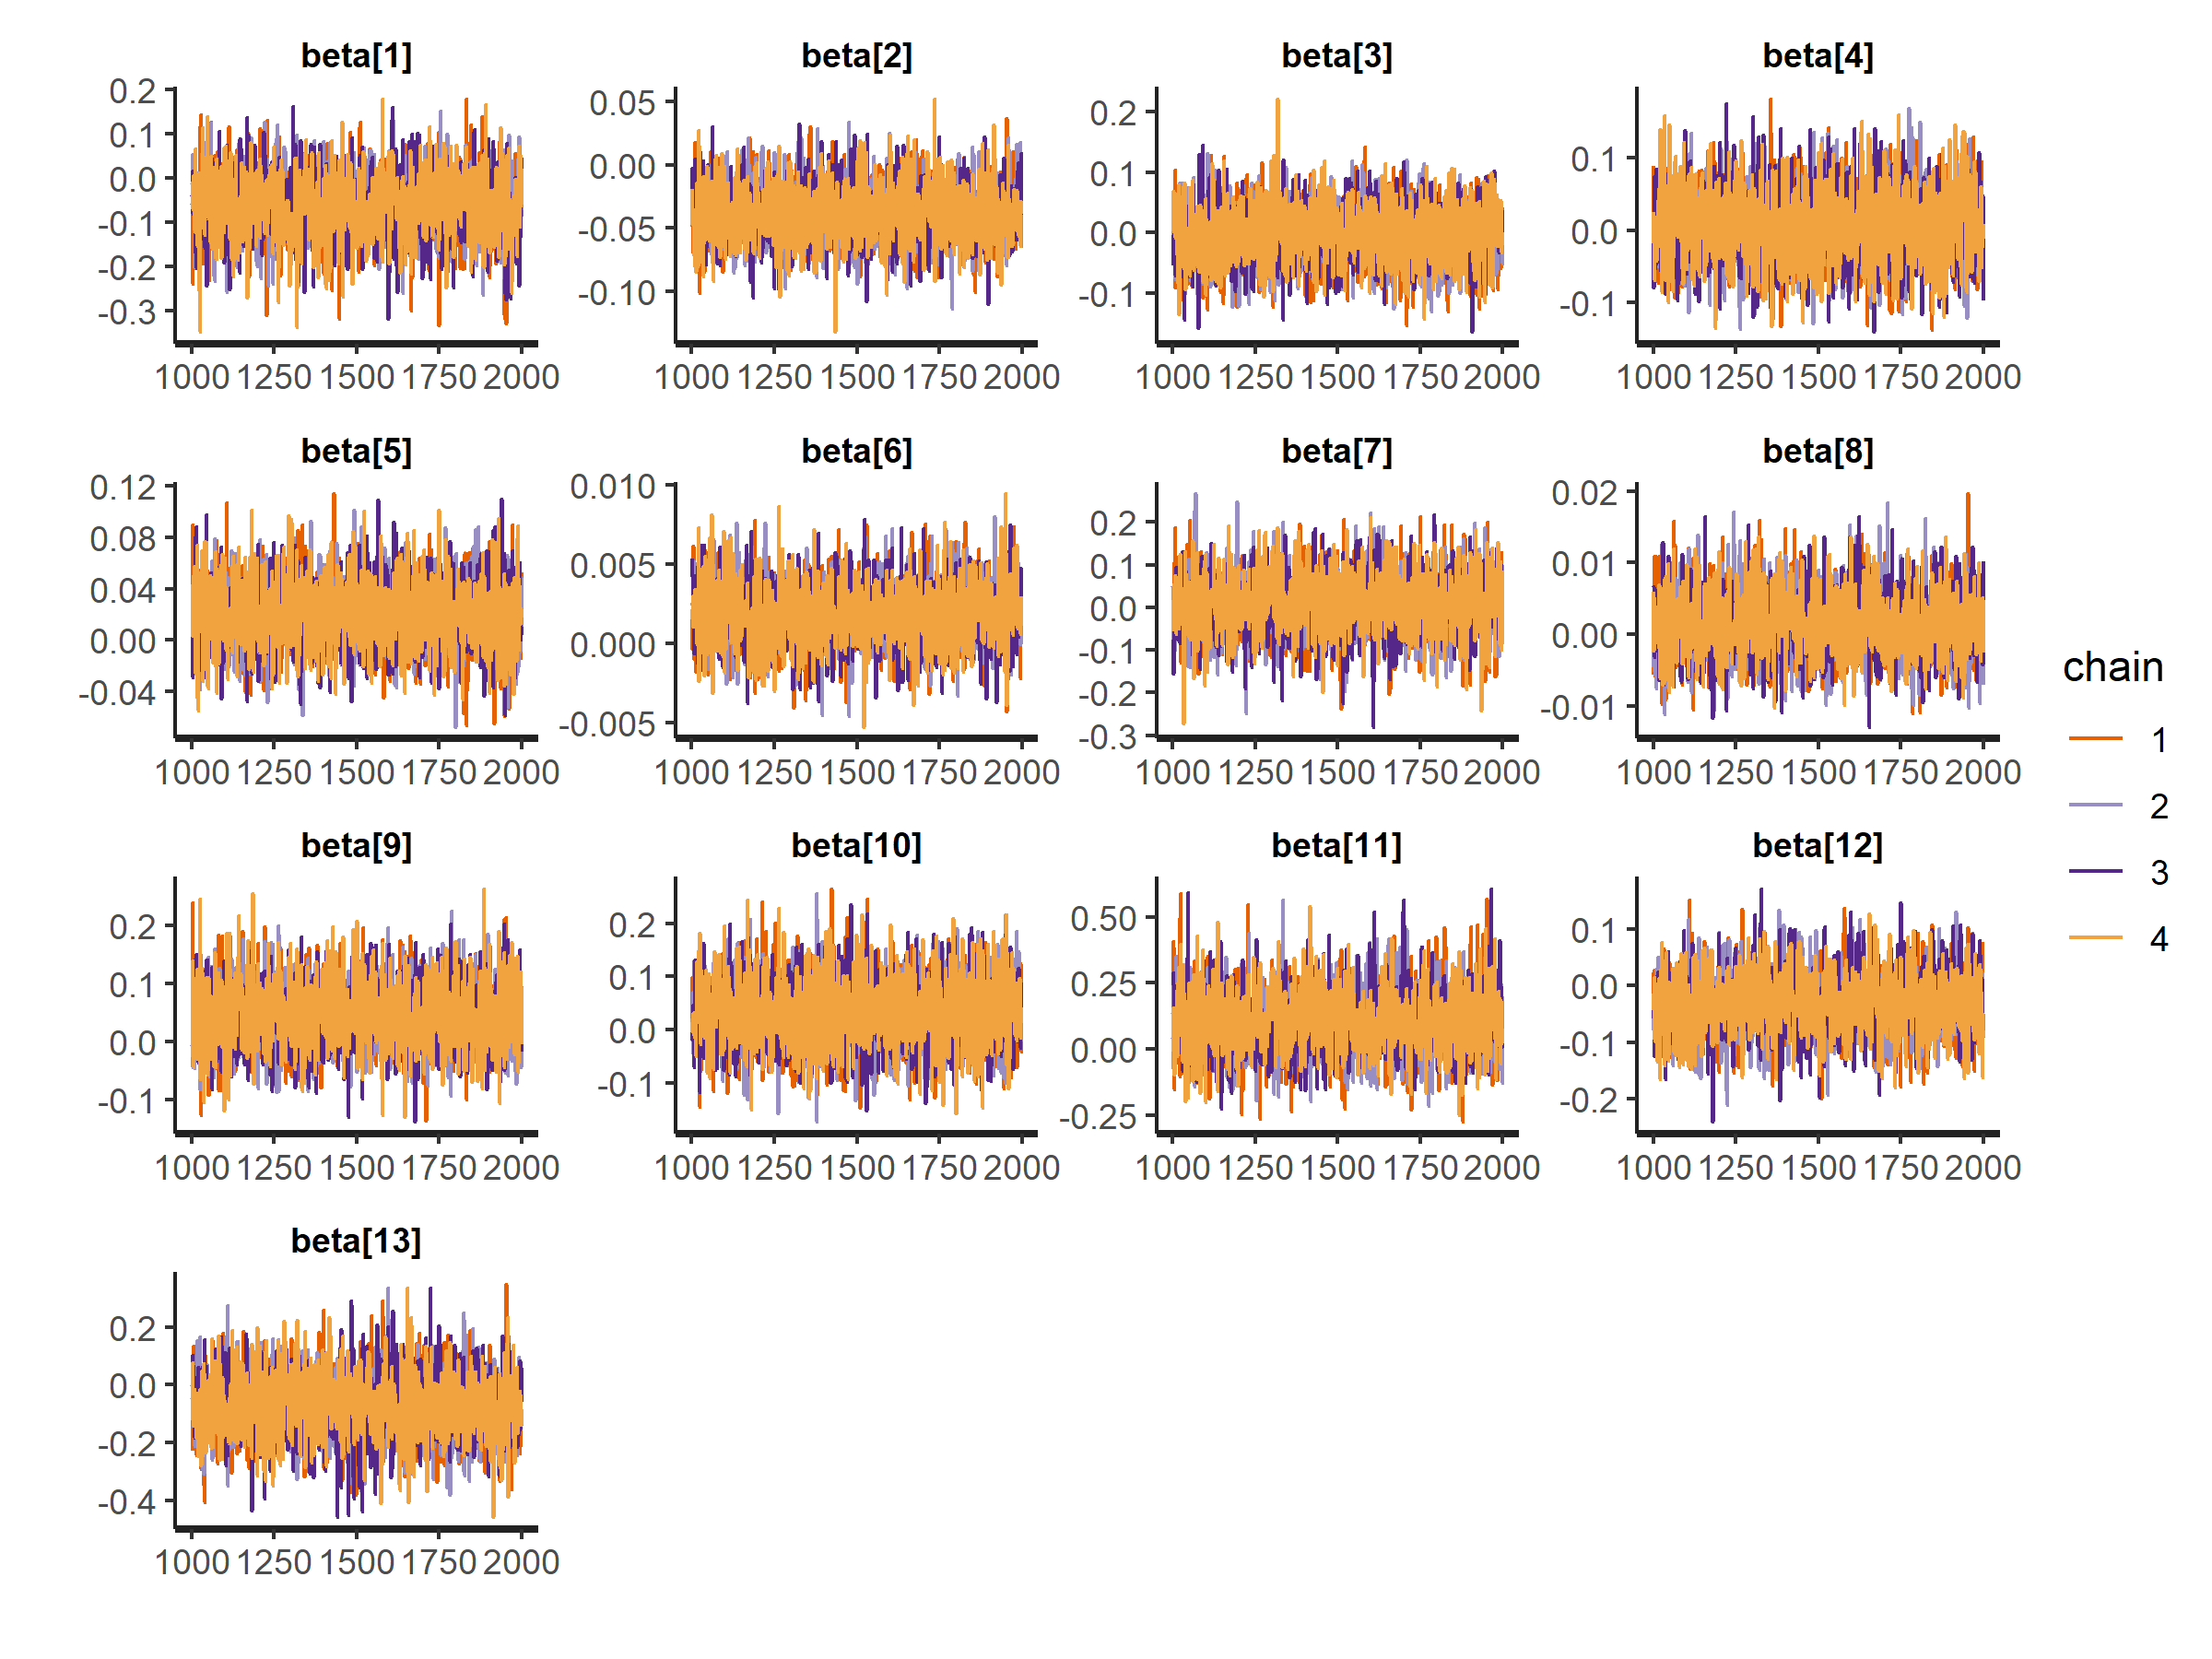
\includegraphics[width=0.95\textwidth]{trace-all-min.png}
	\caption{Traceplot of alliance level parameters in the non-major power sample.}
	\label{fig:trace-all-min}
\end{figure}


\begin{figure}[htbp]
	\centering
		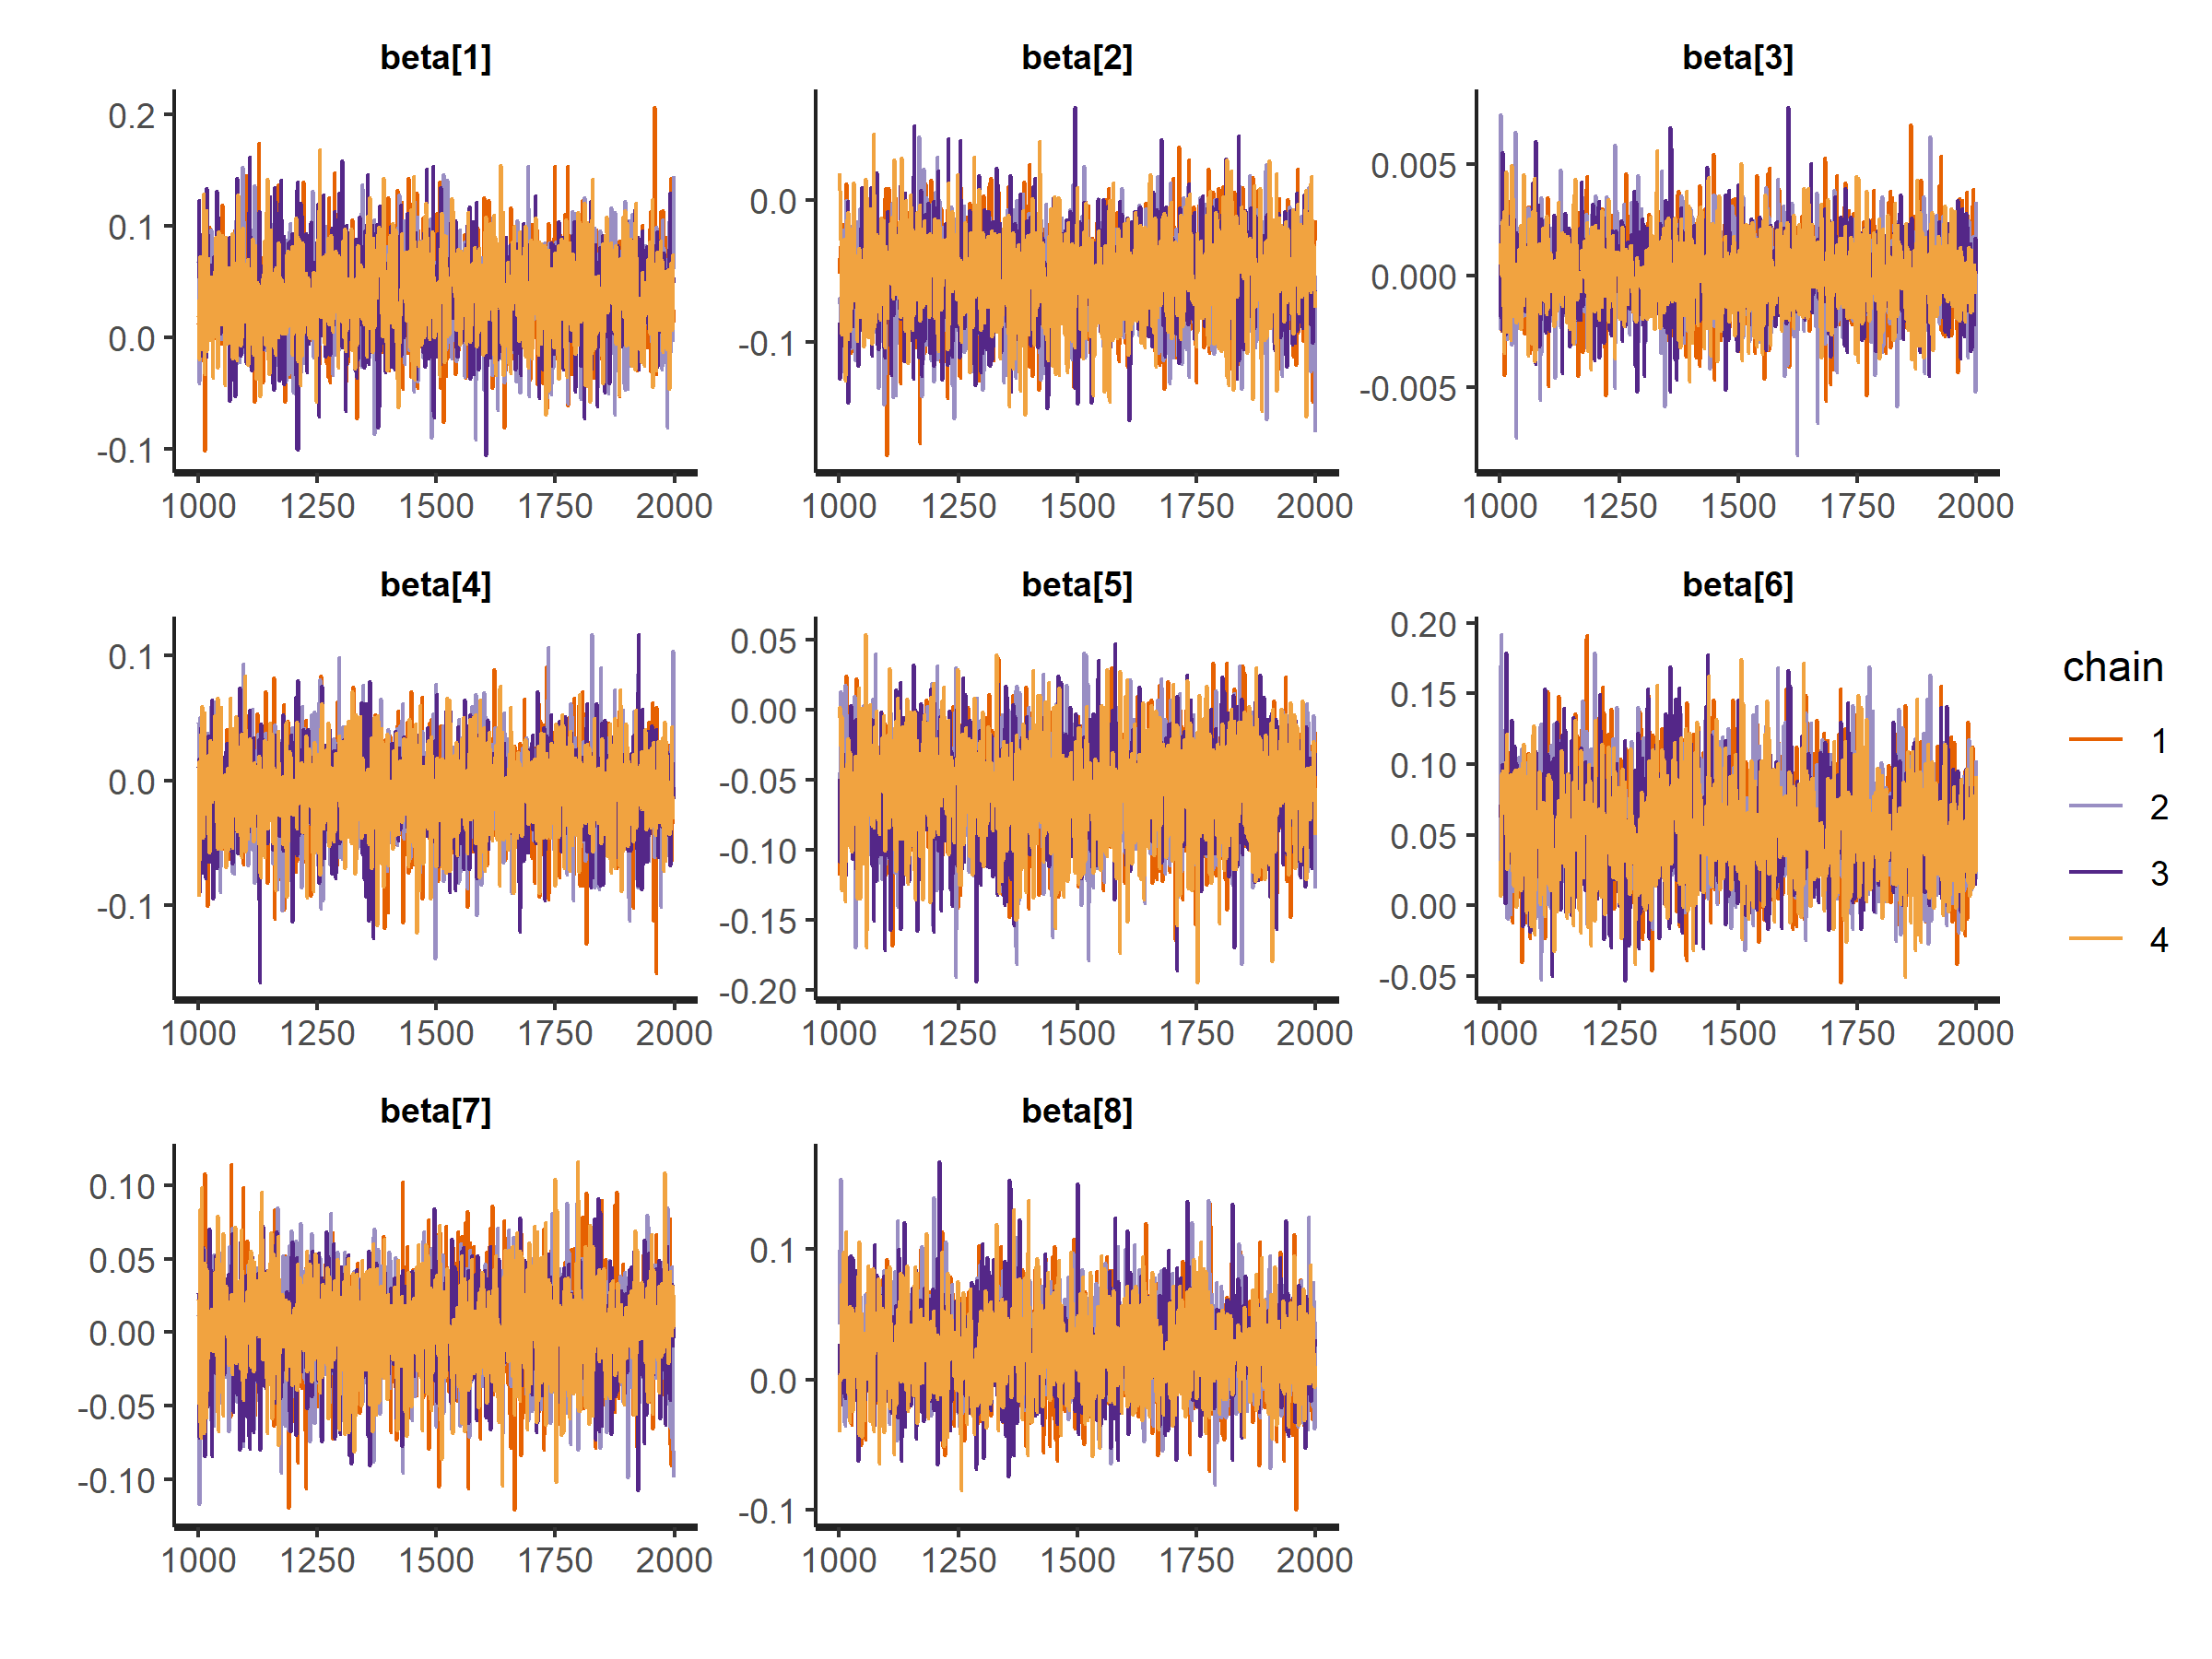
\includegraphics[width=0.95\textwidth]{trace-all-maj.png}
	\caption{Traceplot of alliance level parameters in the major power sample.}
	\label{fig:trace-all-maj}
\end{figure}




\section{Posterior Intervals} 

I do not present tabular summaries of all the alliance-level parameters in the manuscript for parsimony. The next two tables summarize the posteriors of the alliance-level parameters. The use of 90\% credible intervals implies there is a 90\% chance the coefficient is between the 5\% and 95\% values. Because Hypotheses 1 and 2 are directional, I report the positive and negative posterior probabilities in the manuscript.  

\subsection{Major Powers}


\autoref{tab:alliance-level-maj} summarizes the 90\% credible intervals for the alliance parameters in the major power sample, as well as the number of effective samples and $\hat{R}$ for each marginal posterior.\footnote{I report 90\% credible intervals because 95\% interval estimates can be unstable.} $\sigma$ Alliances is the variance hyperparameter for the $\lambda$ estimates. 

The $\hat{R}$ statistics are all close to one, indicating convergence. The number of effective samples is adequate for most parameters. 


\begin{table}[ht]
\centering
\begin{tabular}{rrrrrrr}
  \hline
 & mean & S.D. & 5\% & 95\% & n\_eff & $\hat{R}$ \\ 
  \hline
Constant & 0.038 & 0.038 & -0.025 & 0.102 & 3380.954 & 1.000 \\ 
  Latent Str. & -0.054 & 0.031 & -0.107 & -0.005 & 3278.923 & 1.000 \\ 
  Number Members & 0.000 & 0.002 & -0.003 & 0.003 & 4000.000 & 0.999 \\ 
  Democratic Membership & -0.009 & 0.033 & -0.065 & 0.042 & 4000.000 & 1.000 \\ 
  Wartime & -0.057 & 0.035 & -0.115 & -0.001 & 4000.000 & 1.001 \\ 
  Asymmetric & 0.053 & 0.035 & 0.001 & 0.115 & 2218.509 & 1.000 \\ 
  US Member & 0.002 & 0.031 & -0.051 & 0.051 & 4000.000 & 1.000 \\ 
  USSR Member & 0.023 & 0.033 & -0.028 & 0.079 & 4000.000 & 1.000 \\ 
  $\sigma$ Alliances & 0.066 & 0.029 & 0.019 & 0.117 & 599.081 & 1.007 \\ 
   \hline
\end{tabular}
\caption{90\% Credible intervals for major power alliance-level parameters}
\label{tab:alliance-level-maj}
\end{table}



\subsection{Non-major Powers} 

\autoref{tab:alliance-level-min} summarize the 90\% credible intervals for the alliance-level regression parameters in the non-major power sample. The $\hat{R}$ statistics are all close to one, indicating convergence. The number of effective samples is adequate for all parameters.

\begin{table}[ht]
\centering
\begin{tabular}{rrrrrrr}
  \hline
 & mean & sd & 5\% & 95\% & n\_eff & $\hat{R}$ \\ 
  \hline
Constant & -0.018 & 0.018 & -0.047 & 0.012 & 2211.374 & 1.000 \\ 
  Latent Str. & 0.026 & 0.017 & -0.002 & 0.054 & 2191.382 & 1.000 \\ 
  Number Members & 0.000 & 0.001 & -0.001 & 0.001 & 4000.000 & 1.000 \\ 
  Democratic Membership & -0.031 & 0.015 & -0.056 & -0.009 & 3213.621 & 1.000 \\ 
  Wartime & 0.041 & 0.023 & 0.002 & 0.078 & 4000.000 & 1.000 \\ 
  Asymmetric & -0.031 & 0.021 & -0.065 & 0.003 & 4000.000 & 0.999 \\ 
  US Member & 0.013 & 0.018 & -0.016 & 0.042 & 2895.419 & 1.000 \\ 
  USSR Member & 0.011 & 0.031 & -0.041 & 0.062 & 4000.000 & 1.000 \\ 
  $\sigma$ Alliances & 0.014 & 0.009 & 0.002 & 0.030 & 1254.268 & 1.001 \\ 
   \hline
\end{tabular}
\caption{90\% Credible intervals non-major power alliance-level parameters}
\label{tab:alliance-level-min}
\end{table}


  
% \bibliography{../../MasterBibliography} 




\end{document}
